\documentclass[a4paper,12pt]{article}
\special{papersize=210mm,297mm}

\usepackage[a4paper,top=1.55cm,bottom=1.75cm,left=1.7cm,right=1.7cm]{geometry}
\usepackage[fleqn]{amsmath}
\usepackage{amssymb}
\usepackage{array}
\usepackage{tabularx}
\usepackage{enumitem}
\usepackage{needspace}
\usepackage[hidelinks]{hyperref}
\usepackage{fontspec}
\usepackage{graphicx}
\usepackage{tikz}
\usetikzlibrary{arrows.meta}

\setmainfont{Times New Roman}
\setsansfont{Arial}
\setlength{\parindent}{0pt}
\setlength{\parskip}{0.35em}
\setlength{\mathindent}{1.2em}
\linespread{1.04}
\emergencystretch=2em
\pagestyle{plain}

\newcommand{\examdate}{April 30, 2026}
\newcommand{\problemsection}[2]{%
  \Needspace{8\baselineskip}%
  \phantomsection%
  \section*{Problem #1. #2}%
  \addcontentsline{toc}{section}{Problem #1. #2}%
}
\newcommand{\method}[1]{%
  \Needspace{5\baselineskip}%
  \subsection*{Method #1}%
}
\newcommand{\handin}{%
  \Needspace{5\baselineskip}%
  \subsection*{Clean Hand-in Version}%
}
\newlist{steps}{enumerate}{1}
\setlist[steps]{%
  label=\textbf{Step \arabic*.},
  leftmargin=*,
  itemsep=0.35em,
  topsep=0.35em,
  parsep=0.1em
}
\newlist{subanswers}{enumerate}{1}
\setlist[subanswers]{%
  label=\textbf{(\alph*)},
  leftmargin=*,
  itemsep=0.35em,
  topsep=0.35em,
  parsep=0.1em
}
\newlist{romananswers}{enumerate}{1}
\setlist[romananswers]{%
  label=\textbf{(\roman*)},
  leftmargin=*,
  itemsep=0.35em,
  topsep=0.35em,
  parsep=0.1em
}
\newcommand{\choice}[1]{\(\boxed{\text{#1}}\)}

\newcommand{\contoursaddlefigure}{%
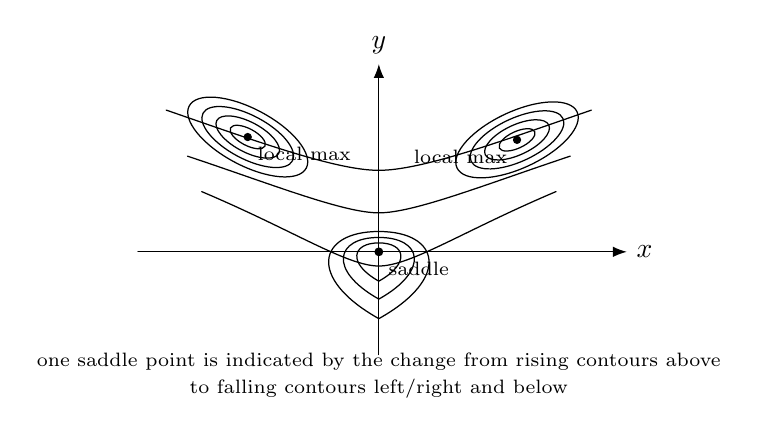
\begin{tikzpicture}[x=0.9cm,y=0.9cm,>=Latex,line cap=round,line join=round]
  \draw[->,line width=0.45pt] (-3.4,0) -- (3.5,0) node[right] {\(x\)};
  \draw[->,line width=0.45pt] (0,-1.45) -- (0,2.65) node[above] {\(y\)};

  \foreach \r in {0.25,0.45,0.65,0.85} {
    \draw[rotate around={-28:(-1.85,1.62)},line width=0.45pt]
      (-1.85,1.62) ellipse[x radius={1.1*\r},y radius={0.47*\r}];
    \draw[rotate around={25:(1.95,1.58)},line width=0.45pt]
      (1.95,1.58) ellipse[x radius={1.1*\r},y radius={0.47*\r}];
  }

  \draw[line width=0.45pt]
    (-3.0,2.0) .. controls (-1.7,1.55) and (-0.6,1.15) .. (0,1.15)
               .. controls (0.6,1.15) and (1.7,1.55) .. (3.0,2.0);
  \draw[line width=0.45pt]
    (-2.7,1.35) .. controls (-1.5,0.95) and (-0.5,0.55) .. (0,0.55)
                .. controls (0.5,0.55) and (1.5,0.95) .. (2.7,1.35);
  \draw[line width=0.45pt]
    (-2.5,0.85) .. controls (-1.2,0.30) and (-0.45,-0.20) .. (0,-0.20)
                .. controls (0.45,-0.20) and (1.2,0.30) .. (2.5,0.85);
  \foreach \r in {0.36,0.58,0.82} {
    \draw[line width=0.45pt]
      (0,{0.35*\r}) .. controls ({-1.05*\r},{0.35*\r}) and ({-1.25*\r},{-0.45*\r}) .. (0,{-1.15*\r})
                     .. controls ({1.25*\r},{-0.45*\r}) and ({1.05*\r},{0.35*\r}) .. (0,{0.35*\r});
  }

  \fill (-1.85,1.62) circle[radius=1.5pt] node[below right] {\scriptsize local max};
  \fill (1.95,1.58) circle[radius=1.5pt] node[below left] {\scriptsize local max};
  \fill (0,0) circle[radius=1.6pt] node[below right] {\scriptsize saddle};
  \node[align=center] at (0,-1.75) {\scriptsize one saddle point is indicated by the change from rising contours above\\[-0.2em]
    \scriptsize to falling contours left/right and below};
\end{tikzpicture}%
}

\newcommand{\cycloidfigure}{%
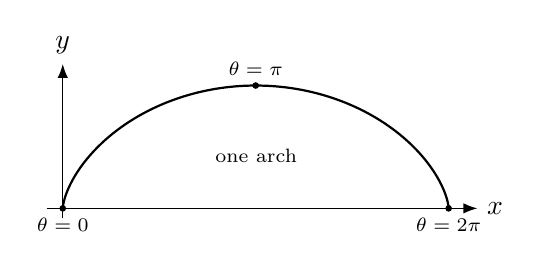
\begin{tikzpicture}[x=0.78cm,y=0.78cm,>=Latex,line cap=round,line join=round]
  \draw[->,line width=0.45pt] (-0.25,0) -- (6.75,0) node[right] {\(x\)};
  \draw[->,line width=0.45pt] (0,-0.15) -- (0,2.35) node[above] {\(y\)};
  \draw[thick]
    plot[domain=0:6.283,samples=220,variable=\t]
      ({\t - sin(\t r)}, {1 - cos(\t r)});
  \fill (0,0) circle[radius=1.2pt] node[below] {\scriptsize \(\theta=0\)};
  \fill (6.283,0) circle[radius=1.2pt] node[below] {\scriptsize \(\theta=2\pi\)};
  \fill (3.1416,2) circle[radius=1.2pt] node[above] {\scriptsize \(\theta=\pi\)};
  \node at (3.15,0.85) {\scriptsize one arch};
\end{tikzpicture}%
}

\newcommand{\polarshadedfigure}{%
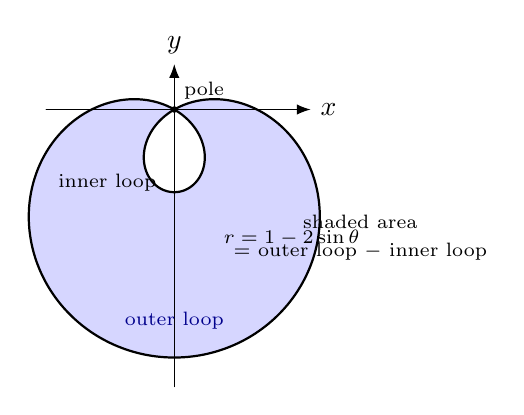
\begin{tikzpicture}[x=1.05cm,y=1.05cm,>=Latex,line cap=round,line join=round]
  \fill[blue!16]
    plot[domain=150:390,samples=260,variable=\t]
      ({(1 - 2*sin(\t))*cos(\t)}, {(1 - 2*sin(\t))*sin(\t)})
    -- cycle;
  \fill[white]
    plot[domain=30:150,samples=160,variable=\t]
      ({(1 - 2*sin(\t))*cos(\t)}, {(1 - 2*sin(\t))*sin(\t)})
    -- cycle;

  \draw[->,line width=0.45pt] (-1.55,0) -- (1.65,0) node[right] {\(x\)};
  \draw[->,line width=0.45pt] (0,-3.35) -- (0,0.55) node[above] {\(y\)};

  \draw[black,thick]
    plot[domain=150:390,samples=260,variable=\t]
      ({(1 - 2*sin(\t))*cos(\t)}, {(1 - 2*sin(\t))*sin(\t)});
  \draw[black,thick]
    plot[domain=30:150,samples=160,variable=\t]
      ({(1 - 2*sin(\t))*cos(\t)}, {(1 - 2*sin(\t))*sin(\t)});

  \fill (0,0) circle[radius=1.2pt] node[above right] {\scriptsize pole};
  \node[right] at (0.48,-1.55) {\scriptsize \(r=1-2\sin\theta\)};
  \node[blue!55!black] at (0,-2.55) {\scriptsize outer loop};
  \node[left] at (-0.10,-0.88) {\scriptsize inner loop};
  \node[align=center] at (2.25,-1.55) {\scriptsize shaded area\\[-0.2em]\scriptsize \(=\) outer loop \(-\) inner loop};
\end{tikzpicture}%
}

\begin{document}

\begin{center}
  {\Large\bfseries Winter Term Calculus Midterm Solutions}\\
  {\large\bfseries Science and Engineering}\\[0.35em]
  Source exam date: April 23, 2026\\
  Solution file date: \examdate
\end{center}

\tableofcontents
\newpage

\problemsection{1}{Maclaurin series and radii of convergence}

\method{1: Use the standard Maclaurin table}

\begin{steps}
\item The Maclaurin series is the Taylor series at \(x=0\):
\[
  f(x)=\sum_{n=0}^{\infty}\frac{f^{(n)}(0)}{n!}x^n.
\]
This is the right starting point because every function in the table is being expanded about \(0\).

\item For \(e^x,\sin x,\cos x\), the derivatives repeat in a simple pattern. Since the factorial in the denominator grows faster than any fixed power of \(x\), these three series converge for every real \(x\), so their radius is \(\infty\).

\item For the rational, logarithmic, inverse tangent, and binomial examples, the nearest singularity to \(0\) is at distance \(1\), unless the binomial series terminates. That explains why their usual radius is \(1\).
\end{steps}

\begin{center}
\renewcommand{\arraystretch}{1.35}
\begin{tabularx}{\linewidth}{|>{\centering\arraybackslash}m{0.18\linewidth}|>{\raggedright\arraybackslash}X|>{\centering\arraybackslash}m{0.16\linewidth}|}
\hline
\textbf{Function} & \centering\arraybackslash\textbf{Maclaurin series} & \textbf{Radius} \\
\hline
\(e^x\) &
\(\displaystyle \sum_{n=0}^{\infty}\dfrac{x^n}{n!}
=1+x+\dfrac{x^2}{2!}+\dfrac{x^3}{3!}+\cdots\)
& \(\infty\)\\
\hline
\(\cos x\) &
\(\displaystyle \sum_{n=0}^{\infty}(-1)^n\dfrac{x^{2n}}{(2n)!}
=1-\dfrac{x^2}{2!}+\dfrac{x^4}{4!}-\cdots\)
& \(\infty\)\\
\hline
\(\dfrac{1}{1+x}\) &
\(\displaystyle \sum_{n=0}^{\infty}(-1)^n x^n
=1-x+x^2-x^3+\cdots\)
& \(1\)\\
\hline
\(\arctan x\) &
\(\displaystyle \sum_{n=0}^{\infty}(-1)^n\dfrac{x^{2n+1}}{2n+1}
=x-\dfrac{x^3}{3}+\dfrac{x^5}{5}-\cdots\)
& \(1\)\\
\hline
\(\ln(1+x)\) &
\(\displaystyle \sum_{n=1}^{\infty}(-1)^{n-1}\dfrac{x^n}{n}
=x-\dfrac{x^2}{2}+\dfrac{x^3}{3}-\cdots\)
& \(1\)\\
\hline
\(\sin x\) &
\(\displaystyle \sum_{n=0}^{\infty}(-1)^n\dfrac{x^{2n+1}}{(2n+1)!}
=x-\dfrac{x^3}{3!}+\dfrac{x^5}{5!}-\cdots\)
& \(\infty\)\\
\hline
\((1+x)^k\) &
\(\displaystyle \sum_{n=0}^{\infty}\binom{k}{n}x^n
=1+kx+\dfrac{k(k-1)}{2!}x^2+\cdots\)
& \(1\), unless \(k=0,1,2,\ldots\)\\
\hline
\end{tabularx}
\end{center}

If \(k\) is a nonnegative integer, the binomial series stops after finitely many terms, so it is a polynomial and its radius of convergence is \(\infty\).

\method{2: Derive the table from generating series}

\begin{steps}
\item Start from the geometric series
\[
  \frac{1}{1-u}=\sum_{n=0}^{\infty}u^n,\qquad |u|<1.
\]
This is useful because several entries can be obtained by substitution or integration.

\item Put \(u=-x\). Then
\[
  \frac{1}{1+x}=\sum_{n=0}^{\infty}(-1)^n x^n,\qquad |x|<1.
\]
The radius is \(1\) because the condition for the geometric series is \(|-x|<1\).

\item Integrate the previous identity from \(0\) to \(x\):
\[
  \ln(1+x)=\int_0^x \frac{1}{1+t}\,dt
  =\sum_{n=0}^{\infty}(-1)^n\frac{x^{n+1}}{n+1}.
\]
Term-by-term integration is appropriate inside the interval of convergence.

\item Use
\[
  \frac{1}{1+x^2}=\sum_{n=0}^{\infty}(-1)^n x^{2n}
\]
and integrate:
\[
  \arctan x=\int_0^x\frac{1}{1+t^2}\,dt
  =\sum_{n=0}^{\infty}(-1)^n\frac{x^{2n+1}}{2n+1}.
\]

\item The series for \(e^x,\sin x,\cos x\) come directly from the derivative pattern in Taylor's formula. The generalized binomial theorem gives
\[
  (1+x)^k=\sum_{n=0}^{\infty}\binom{k}{n}x^n,\qquad
  \binom{k}{n}=\frac{k(k-1)\cdots(k-n+1)}{n!}.
\]
\end{steps}

\problemsection{2}{Vectors normal to \(\langle 1,2,3\rangle\)}

\method{1: Dot products}

\begin{steps}
\item Two vectors are normal when their dot product is \(0\). This is the correct test because the dot product measures the component of one vector in the direction of the other.

\item Compute each dot product with \(\langle 1,2,3\rangle\):
\[
\begin{array}{c|c}
\text{candidate vector} & \text{dot product with }\langle 1,2,3\rangle\\
\hline
\langle 3,0,-1\rangle & 3+0-3=0\\
\langle 1,-2,1\rangle & 1-4+3=0\\
\langle 0,-3,2\rangle & 0-6+6=0\\
\langle 4,-2,0\rangle & 4-4+0=0\\
\langle 1,-1,1\rangle & 1-2+3=2
\end{array}
\]

\item Therefore the first four vectors are normal, and the last vector is not.
\end{steps}

\method{2: Use the normal-vector equation}

\begin{steps}
\item A vector \(\langle a,b,c\rangle\) is normal to \(\langle 1,2,3\rangle\) exactly when
\[
  \langle a,b,c\rangle\cdot \langle 1,2,3\rangle=a+2b+3c=0.
\]
This equation describes the plane through the origin perpendicular to \(\langle 1,2,3\rangle\).

\item Substitute each candidate into \(a+2b+3c=0\). The first four satisfy the equation, but
\[
  1+2(-1)+3(1)=2\ne0
\]
for \(\langle 1,-1,1\rangle\).
\end{steps}

\problemsection{3}{Multiple choice problems}

\method{1: Direct tests and definitions}

\begin{romananswers}
\item The contour map shows one saddle point, at the marked point near the origin. The two upper marked points are surrounded by closed contours whose values increase inward, so they represent local maxima, not saddles.

\begin{center}
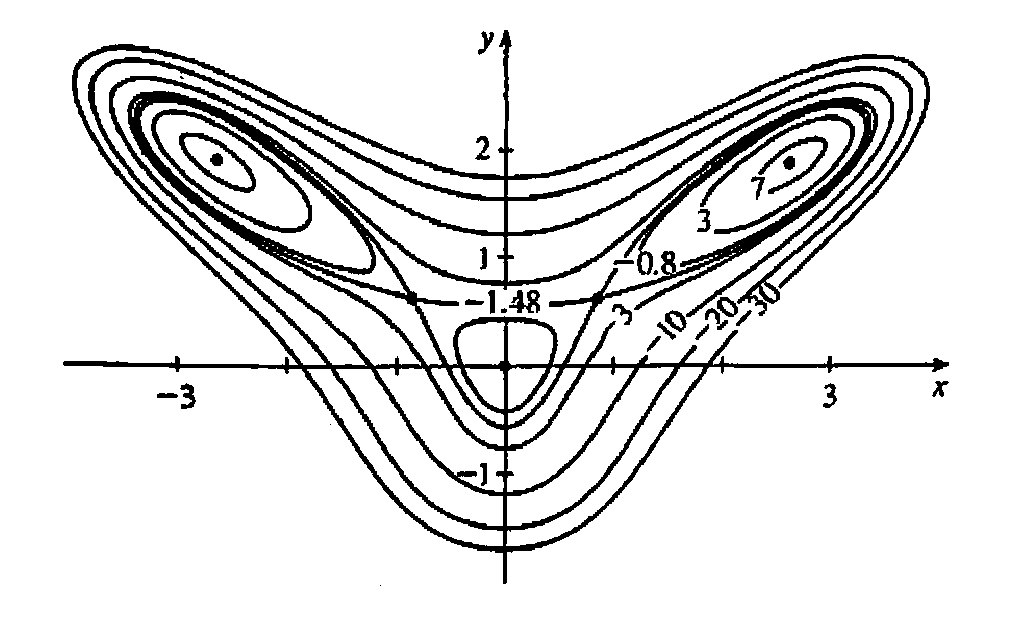
\includegraphics[width=7.6cm]{3i.png}
\end{center}

Thus the answer is \(\boxed{1}\), choice \choice{B}.

\item For
\[
  \sum_{n=0}^{\infty}(-1)^n\frac{n}{\sqrt{3n^2+n-3}},
\]
the terms must approach \(0\) if the series is to converge. But for large \(n\),
\[
  \frac{n}{\sqrt{3n^2+n-3}}
  =\frac{1}{\sqrt{3+1/n-3/n^2}}
  \longrightarrow \frac{1}{\sqrt3}.
\]
The terms oscillate near \(\pm 1/\sqrt3\), so the terms do not approach \(0\). Therefore the series diverges, choice \choice{C}. The printed \(n=0\) term is not real, but the tail already forces divergence.

\item For
\[
  \sum_{n=2}^{\infty}\frac{(-1)^n}{n(\ln n)^2},
\]
check absolute convergence:
\[
  \sum_{n=2}^{\infty}\left|\frac{(-1)^n}{n(\ln n)^2}\right|
  =\sum_{n=2}^{\infty}\frac{1}{n(\ln n)^2}.
\]
The integral test gives
\[
  \int_2^\infty \frac{dx}{x(\ln x)^2}
  =\left[-\frac{1}{\ln x}\right]_2^\infty
  =\frac{1}{\ln2}<\infty.
\]
Hence the series is absolutely convergent, choice \choice{A}.

\item Since \(\cos(n\pi)=(-1)^n\),
\[
  \sum_{n=1}^{\infty}\frac{\cos(n\pi)}{n}
  =\sum_{n=1}^{\infty}\frac{(-1)^n}{n}.
\]
This converges by the alternating-series test because \(1/n\) decreases to \(0\). However,
\[
  \sum_{n=1}^{\infty}\left|\frac{(-1)^n}{n}\right|
  =\sum_{n=1}^{\infty}\frac{1}{n}
\]
diverges. Thus the series is conditionally convergent, choice \choice{B}.

\item For
\[
  \sum_{n=1}^{\infty}(-1)^n\frac{100^n}{n!},
\]
test absolute convergence:
\[
  a_n=\frac{100^n}{n!},\qquad
  \frac{a_{n+1}}{a_n}
  =\frac{100}{n+1}\to0<1.
\]
The ratio test gives absolute convergence, choice \choice{A}.

\item[(xiii)] Use the definition
\[
  \binom{1/2}{4}
  =\frac{(1/2)(1/2-1)(1/2-2)(1/2-3)}{4!}.
\]
Thus
\[
  \binom{1/2}{4}
  =\frac{(1/2)(-1/2)(-3/2)(-5/2)}{24}
  =-\frac{15}{16\cdot24}
  =-\frac{5}{128}
  =-\frac{5}{2^7}.
\]
The answer is choice \choice{H}.
\end{romananswers}

\method{2: Alternate recognitions}

\begin{romananswers}
\item In a vertical slice through the origin, the contour values increase as we move upward toward the positive labeled contours; in a horizontal slice, nearby labeled contours decrease away from the origin. Increasing in one direction and decreasing in a transverse direction is the geometric signature of a saddle. The upper two dots have closed contour nests, so they are extrema. Therefore there is one saddle point.

\item The even subsequence of terms tends to \(1/\sqrt3\), while the odd subsequence tends to \(-1/\sqrt3\). Since a convergent series must have terms with every subsequence tending to \(0\), this series is divergent.

\item Cauchy's condensation test gives another way to check the absolute-value series. For
\[
  b_n=\frac{1}{n(\ln n)^2},
\]
the condensed series has terms
\[
  2^m b_{2^m}
  =\frac{1}{(\ln 2^m)^2}
  =\frac{1}{m^2(\ln2)^2}.
\]
This is a constant multiple of a convergent \(p\)-series with \(p=2\), so the original absolute-value series converges.

\item The known Taylor value
\[
  \ln2=\sum_{n=1}^{\infty}\frac{(-1)^{n-1}}{n}
\]
shows that
\[
  \sum_{n=1}^{\infty}\frac{(-1)^n}{n}=-\ln2
\]
converges. Since the absolute-value series is the harmonic series, the convergence is conditional.

\item The absolute-value series is recognized as part of the exponential series:
\[
  \sum_{n=1}^{\infty}\frac{100^n}{n!}=e^{100}-1<\infty.
\]
Therefore the original alternating series is absolutely convergent.

\item[(xiii)] The recurrence
\[
  \binom{\alpha}{m+1}=\binom{\alpha}{m}\frac{\alpha-m}{m+1}
\]
with \(\alpha=\frac12\) gives
\[
  \binom{1/2}{1}=\frac12,\quad
  \binom{1/2}{2}=-\frac18,\quad
  \binom{1/2}{3}=\frac1{16},\quad
  \binom{1/2}{4}=-\frac5{128}.
\]
\end{romananswers}

\problemsection{4}{The tenth derivative of \((1-2x^2)^{-5}\)}

\method{1: Generalized binomial expansion}

\begin{steps}
\item Write the function in binomial form:
\[
  f(x)=(1-2x^2)^{-5}.
\]
This is appropriate because the exponent \(-5\) and the expression \(1+\text{something}\) match the generalized binomial theorem.

\item Use
\[
  (1+u)^\alpha=\sum_{m=0}^{\infty}\binom{\alpha}{m}u^m.
\]
With \(\alpha=-5\) and \(u=-2x^2\),
\[
  f(x)=\sum_{m=0}^{\infty}\binom{-5}{m}(-2x^2)^m.
\]

\item The tenth derivative at \(0\) depends only on the coefficient of \(x^{10}\). Since \(x^{2m}=x^{10}\) when \(m=5\), the relevant term is
\[
  \binom{-5}{5}(-2)^5x^{10}
  =-\binom{-5}{5}2^5x^{10}.
\]

\item If \(f(x)=\sum c_jx^j\), then \(f^{(10)}(0)=10!c_{10}\). Therefore
\[
  f^{(10)}(0)
  =10!\left[-\binom{-5}{5}2^5\right]
  =(-10!)\binom{-5}{5}2^5.
\]
Matching
\[
  f^{(10)}(0)=a\binom{-5}{k}2^n
\]
gives
\[
  \boxed{a=-10!},\qquad \boxed{k=5},\qquad \boxed{n=5}.
\]
\end{steps}

\method{2: Positive-coefficient form, then convert}

\begin{steps}
\item Use the negative-binomial identity
\[
  \frac{1}{(1-z)^5}=\sum_{m=0}^{\infty}\binom{m+4}{4}z^m.
\]
This form is useful because \(1/(1-z)^5\) has positive coefficients.

\item Put \(z=2x^2\):
\[
  f(x)=\sum_{m=0}^{\infty}\binom{m+4}{4}2^m x^{2m}.
\]
Again \(x^{10}\) occurs when \(m=5\), so
\[
  c_{10}=\binom{9}{4}2^5.
\]

\item Therefore
\[
  f^{(10)}(0)=10!\binom{9}{4}2^5.
\]
To match the requested form, use
\[
  \binom{-5}{5}=(-1)^5\binom{9}{5}=-\binom{9}{4}.
\]
So
\[
  10!\binom{9}{4}2^5
  =(-10!)\binom{-5}{5}2^5.
\]
\end{steps}

\problemsection{5}{Error bound for \(\sin x\approx x-x^3/{3!}+x^5/{5!}\)}

\method{1: Alternating-series remainder}

\begin{steps}
\item The Maclaurin series for sine is
\[
  \sin x=x-\frac{x^3}{3!}+\frac{x^5}{5!}-\frac{x^7}{7!}+\cdots.
\]
The given approximation stops after the \(x^5\) term.

\item For \(|x|<0.2\), the magnitudes
\[
  \frac{|x|^{2n+1}}{(2n+1)!}
\]
decrease. This lets us use the alternating-series error estimate: the error is at most the magnitude of the next omitted term.

\item The next omitted term is \(x^7/{7!}\), so
\[
  |R|\le \frac{|x|^7}{7!}<\frac{0.2^7}{7!}
  =\frac{0.0000128}{5040}
  \approx 2.54\times10^{-9}.
\]
\end{steps}

\method{2: Taylor's theorem}

\begin{steps}
\item The given polynomial is also the Taylor polynomial for \(\sin x\) through degree \(6\), because the \(x^6\) coefficient is \(0\). This is useful because Taylor's theorem with remainder then uses the seventh derivative.

\item Taylor's theorem gives
\[
  R_6(x)=\frac{f^{(7)}(\xi)}{7!}x^7
\]
for some \(\xi\) between \(0\) and \(x\).

\item Since \(f(x)=\sin x\), we have \(f^{(7)}(x)=-\cos x\). Therefore
\[
  |f^{(7)}(\xi)|=|\cos\xi|\le1.
\]
Thus
\[
  |R_6(x)|\le\frac{|x|^7}{7!}<\frac{0.2^7}{7!}.
\]
\end{steps}

\problemsection{6}{Maclaurin series for \(x\sin x\) and the given sum}

\method{1: Multiply the sine series, then integrate}

\begin{subanswers}
\item The sine series is
\[
  \sin x=\sum_{n=0}^{\infty}(-1)^n\frac{x^{2n+1}}{(2n+1)!}.
\]
Multiplying by \(x\) is appropriate because \(x\sin x\) is exactly \(x\) times the known series:
\[
  x\sin x
  =\sum_{n=0}^{\infty}(-1)^n\frac{x^{2n+2}}{(2n+1)!}.
\]
The sine series has infinite radius of convergence, and multiplying by \(x\) does not change that. Hence the interval of convergence is
\[
  \boxed{(-\infty,\infty)}.
\]

\item Integrate from \(0\) to \(\pi\). Term-by-term integration is allowed because the power series has infinite radius of convergence:
\[
  \int_0^\pi x\sin x\,dx
  =
  \sum_{n=0}^{\infty}
  \frac{(-1)^n\pi^{2n+3}}{(2n+1)!(2n+3)}.
\]
Now evaluate the integral:
\[
  \int_0^\pi x\sin x\,dx
  =[-x\cos x+\sin x]_0^\pi
  =\pi.
\]
Thus
\[
  \sum_{n=0}^{\infty}
  \frac{(-1)^n\pi^{2n+3}}{(2n+1)!(2n+3)}
  =\pi.
\]
Dividing by \(\pi\) gives
\[
  \boxed{
  \sum_{n=0}^{\infty}
  \frac{(-1)^n\pi^{2n+2}}{(2n+1)!(2n+3)}
  =1 }.
\]
\end{subanswers}

\method{2: Build the target sum directly}

\begin{steps}
\item Notice that the denominator \(2n+3\) is what appears when integrating \(x^{2n+2}\):
\[
  \int_0^\pi x^{2n+2}\,dx=\frac{\pi^{2n+3}}{2n+3}.
\]
This observation tells us that the target sum should come from an integral of the series for \(x\sin x\).

\item Define
\[
  S=\sum_{n=0}^{\infty}
  \frac{(-1)^n\pi^{2n+2}}{(2n+1)!(2n+3)}.
\]
Multiplying by \(\pi\),
\[
  \pi S=
  \sum_{n=0}^{\infty}
  \frac{(-1)^n\pi^{2n+3}}{(2n+1)!(2n+3)}
  =
  \int_0^\pi
  \sum_{n=0}^{\infty}(-1)^n\frac{x^{2n+2}}{(2n+1)!}\,dx.
\]

\item The series inside the integral is \(x\sin x\), so
\[
  \pi S=\int_0^\pi x\sin x\,dx=\pi.
\]
Therefore \(S=1\).
\end{steps}

\problemsection{7}{Cycloid}

\[
  x=\theta-\sin\theta,\qquad y=1-\cos\theta.
\]

\begin{center}
\cycloidfigure{}
\end{center}

\method{1: Parametric differentiation}

\begin{subanswers}
\item First compute
\[
  \frac{dx}{d\theta}=1-\cos\theta,\qquad
  \frac{dy}{d\theta}=\sin\theta.
\]
For a parametric curve, the slope is
\[
  \frac{dy}{dx}
  =
  \frac{dy/d\theta}{dx/d\theta}
  =
  \frac{\sin\theta}{1-\cos\theta}.
\]
Using half-angle identities,
\[
  \frac{\sin\theta}{1-\cos\theta}
  =
  \frac{2\sin(\theta/2)\cos(\theta/2)}
       {2\sin^2(\theta/2)}
  =
  \boxed{\cot\frac{\theta}{2}}.
\]

\item For the second derivative,
\[
  \frac{d^2y}{dx^2}
  =
  \frac{d}{d\theta}\left(\frac{dy}{dx}\right)
  \bigg/ \frac{dx}{d\theta}.
\]
This formula is appropriate because \(dy/dx\) is still a function of \(\theta\). Since
\[
  \frac{dy}{dx}=\frac{\sin\theta}{1-\cos\theta},
\]
we get
\[
  \frac{d}{d\theta}\left(\frac{\sin\theta}{1-\cos\theta}\right)
  =
  \frac{\cos\theta(1-\cos\theta)-\sin^2\theta}{(1-\cos\theta)^2}
  =
  -\frac{1}{1-\cos\theta}.
\]
Therefore
\[
  \frac{d^2y}{dx^2}
  =
  \frac{-1/(1-\cos\theta)}{1-\cos\theta}
  =
  \boxed{-\frac{1}{(1-\cos\theta)^2}}.
\]

\item One arch is traced by \(0\le\theta\le2\pi\). The parametric arc length formula gives
\[
  L=\int_0^{2\pi}
  \sqrt{\left(\frac{dx}{d\theta}\right)^2+
        \left(\frac{dy}{d\theta}\right)^2}\,d\theta.
\]
Substitute the derivatives:
\[
  L=\int_0^{2\pi}
  \sqrt{(1-\cos\theta)^2+\sin^2\theta}\,d\theta.
\]
Simplify the integrand:
\[
  (1-\cos\theta)^2+\sin^2\theta
  =1-2\cos\theta+\cos^2\theta+\sin^2\theta
  =2-2\cos\theta
  =4\sin^2\frac{\theta}{2}.
\]
Since \(0\le\theta\le2\pi\), \(\sin(\theta/2)\ge0\), so
\[
  \boxed{L=\int_0^{2\pi}2\sin\frac{\theta}{2}\,d\theta}.
\]
If evaluated, this equals \(8\).
\end{subanswers}

\method{2: Use the half-angle form of the tangent vector}

\begin{steps}
\item Rewrite the tangent vector:
\[
  \left(\frac{dx}{d\theta},\frac{dy}{d\theta}\right)
  =(1-\cos\theta,\sin\theta)
  =
  \left(2\sin^2\frac{\theta}{2},
  2\sin\frac{\theta}{2}\cos\frac{\theta}{2}\right).
\]
This form is useful because both components share the factor \(2\sin(\theta/2)\).

\item The slope is the ratio of the second component to the first:
\[
  \frac{dy}{dx}
  =
  \frac{2\sin(\theta/2)\cos(\theta/2)}
       {2\sin^2(\theta/2)}
  =
  \cot\frac{\theta}{2}.
\]

\item Differentiate \(\cot(\theta/2)\) with respect to \(\theta\), then divide by \(dx/d\theta=2\sin^2(\theta/2)\):
\[
  \frac{d^2y}{dx^2}
  =
  \frac{-\frac12\csc^2(\theta/2)}
       {2\sin^2(\theta/2)}
  =
  -\frac{1}{4\sin^4(\theta/2)}
  =
  -\frac{1}{(1-\cos\theta)^2}.
\]

\item The speed is the length of the tangent vector:
\[
  \sqrt{\left(2\sin^2\frac{\theta}{2}\right)^2+
        \left(2\sin\frac{\theta}{2}\cos\frac{\theta}{2}\right)^2}
  =
  2\sin\frac{\theta}{2}.
\]
So the arc length of one arch is again
\[
  \int_0^{2\pi}2\sin\frac{\theta}{2}\,d\theta.
\]
\end{steps}

\problemsection{8}{Limit and continuity at the origin}

\[
f(x,y)=
\begin{cases}
\dfrac{xy}{x^2+y^2}, & (x,y)\ne(0,0),\\[0.6em]
0, & (x,y)=(0,0).
\end{cases}
\]

\method{1: Compare paths}

\begin{subanswers}
\item Approach along the line \(y=x\):
\[
  f(x,x)=\frac{x^2}{x^2+x^2}=\frac12.
\]
Approach along the line \(y=-x\):
\[
  f(x,-x)=\frac{-x^2}{x^2+x^2}=-\frac12.
\]
These two paths approach the same point \((0,0)\), but they give different limiting values. Therefore
\[
  \lim_{(x,y)\to(0,0)}f(x,y)\text{ does not exist}.
\]

\item A function is continuous at \((0,0)\) only if the limit exists and equals \(f(0,0)\). Here the limit does not exist, so \(f\) is not continuous at \((0,0)\).
\end{subanswers}

\method{2: Polar coordinates}

\begin{steps}
\item Put \(x=r\cos\theta\) and \(y=r\sin\theta\). For \(r\ne0\),
\[
  f(x,y)
  =
  \frac{r^2\cos\theta\sin\theta}{r^2}
  =
  \cos\theta\sin\theta
  =
  \frac12\sin2\theta.
\]

\item A limit as \((x,y)\to(0,0)\) must be independent of direction. But the expression \(\frac12\sin2\theta\) depends on \(\theta\). For example, \(\theta=\pi/4\) gives \(1/2\), while \(\theta=-\pi/4\) gives \(-1/2\).

\item Therefore the limit does not exist, and the function is not continuous at the origin.
\end{steps}

\problemsection{9}{Polar curve \(r=1-2\sin\theta\)}

\begin{center}
\polarshadedfigure{}
\end{center}

\method{1: Polar derivative formula and loop intervals}

\begin{subanswers}
\item For a polar curve,
\[
  x=r\cos\theta,\qquad y=r\sin\theta,
\]
so
\[
  \frac{dy}{dx}
  =
  \frac{dy/d\theta}{dx/d\theta}
  =
  \frac{r' \sin\theta+r\cos\theta}
       {r'\cos\theta-r\sin\theta}.
\]
Here
\[
  r=1-2\sin\theta,\qquad r'=-2\cos\theta.
\]
Therefore
\[
  \frac{dy}{dx}
  =
  \frac{(-2\cos\theta)\sin\theta+(1-2\sin\theta)\cos\theta}
       {(-2\cos\theta)\cos\theta-(1-2\sin\theta)\sin\theta}.
\]
Simplifying,
\[
  \boxed{
  \frac{dy}{dx}
  =
  \frac{\cos\theta(1-4\sin\theta)}
       {4\sin^2\theta-\sin\theta-2}}
\]
where the denominator is not zero.

\item The curve has \(r=0\) when
\[
  1-2\sin\theta=0
  \quad\Longrightarrow\quad
  \sin\theta=\frac12,
\]
so
\[
  \theta=\frac{\pi}{6},\quad \frac{5\pi}{6}.
\]
The inner loop is traced on
\[
  \frac{\pi}{6}\le\theta\le\frac{5\pi}{6},
\]
and the outer loop is traced on
\[
  \frac{5\pi}{6}\le\theta\le\frac{13\pi}{6}.
\]
The polar area formula is
\[
  A=\frac12\int r^2\,d\theta.
\]
Since the shaded region is inside the outer loop but outside the inner loop,
\[
  \boxed{
  A=
  \frac12\int_{5\pi/6}^{13\pi/6}(1-2\sin\theta)^2\,d\theta
  -
  \frac12\int_{\pi/6}^{5\pi/6}(1-2\sin\theta)^2\,d\theta}.
\]
\end{subanswers}

\method{2: Differentiate \(x(\theta)\), \(y(\theta)\), then evaluate the area if desired}

\begin{steps}
\item Write the curve parametrically:
\[
  x=(1-2\sin\theta)\cos\theta,\qquad
  y=(1-2\sin\theta)\sin\theta.
\]
Differentiating directly gives
\[
  \frac{dx}{d\theta}
  =
  -2\cos^2\theta-(1-2\sin\theta)\sin\theta,
\]
\[
  \frac{dy}{d\theta}
  =
  -2\cos\theta\sin\theta+(1-2\sin\theta)\cos\theta.
\]
The ratio \((dy/d\theta)/(dx/d\theta)\) gives the same slope formula as Method 1.

\item For the area, expand
\[
  (1-2\sin\theta)^2
  =1-4\sin\theta+4\sin^2\theta
  =3-4\sin\theta-2\cos2\theta.
\]
An antiderivative is
\[
  3\theta+4\cos\theta-\sin2\theta.
\]

\item Thus the outer loop area is
\[
  \frac12\left[3\theta+4\cos\theta-\sin2\theta\right]_{5\pi/6}^{13\pi/6}
  =2\pi+\frac{3\sqrt3}{2},
\]
and the inner loop area is
\[
  \frac12\left[3\theta+4\cos\theta-\sin2\theta\right]_{\pi/6}^{5\pi/6}
  =\pi-\frac{3\sqrt3}{2}.
\]
Therefore the shaded area would be
\[
  \left(2\pi+\frac{3\sqrt3}{2}\right)
  -
  \left(\pi-\frac{3\sqrt3}{2}\right)
  =
  \pi+3\sqrt3.
\]
The problem only asks to set up the definite integral, but this value checks the setup.
\end{steps}

\newpage
\section*{Final Clean Hand-in Answers}
\addcontentsline{toc}{section}{Final Clean Hand-in Answers}

\begin{enumerate}[label=\textbf{\arabic*.},leftmargin=*]
\item
\[
\begin{array}{|c|c|c|}
\hline
\text{Function} & \text{Maclaurin series} & \text{Radius}\\
\hline
e^x & \displaystyle \sum_{n=0}^{\infty}\frac{x^n}{n!} & \infty\\
\hline
\cos x & \displaystyle \sum_{n=0}^{\infty}(-1)^n\frac{x^{2n}}{(2n)!} & \infty\\
\hline
\dfrac{1}{1+x} & \displaystyle \sum_{n=0}^{\infty}(-1)^n x^n & 1\\
\hline
\arctan x & \displaystyle \sum_{n=0}^{\infty}(-1)^n\frac{x^{2n+1}}{2n+1} & 1\\
\hline
\ln(1+x) & \displaystyle \sum_{n=1}^{\infty}(-1)^{n-1}\frac{x^n}{n} & 1\\
\hline
\sin x & \displaystyle \sum_{n=0}^{\infty}(-1)^n\frac{x^{2n+1}}{(2n+1)!} & \infty\\
\hline
(1+x)^k & \displaystyle \sum_{n=0}^{\infty}\binom{k}{n}x^n & 1\text{ unless the series terminates}\\
\hline
\end{array}
\]

\item The normal vectors are
\[
  \boxed{\langle3,0,-1\rangle,\quad
  \langle1,-2,1\rangle,\quad
  \langle0,-3,2\rangle,\quad
  \langle4,-2,0\rangle}.
\]

\item
\[
\begin{array}{c|c|c}
\text{subpart} & \text{answer} & \text{choice}\\
\hline
(i) & 1\text{ saddle point} & B\\
(ii) & \text{divergent} & C\\
(iii) & \text{absolutely convergent} & A\\
(iv) & \text{conditionally convergent} & B\\
(v) & \text{absolutely convergent} & A\\
(xiii) & \displaystyle -\frac{5}{2^7} & H
\end{array}
\]

\item
\[
  f^{(10)}(0)=(-10!)\binom{-5}{5}2^5,
\]
so
\[
  \boxed{a=-10!},\qquad \boxed{k=5},\qquad \boxed{n=5}.
\]

\item
\[
  \left|\sin x-\left(x-\frac{x^3}{3!}+\frac{x^5}{5!}\right)\right|
  \le\frac{|x|^7}{7!}
  <\boxed{\frac{0.2^7}{7!}\approx2.54\times10^{-9}}.
\]

\item
\begin{enumerate}[label=\textbf{(\alph*)},leftmargin=*]
\item
\[
  x\sin x=\sum_{n=0}^{\infty}(-1)^n\frac{x^{2n+2}}{(2n+1)!},
  \qquad \text{interval }(-\infty,\infty).
\]
\item
\[
  \int_0^\pi x\sin x\,dx=\pi
  =
  \sum_{n=0}^{\infty}
  \frac{(-1)^n\pi^{2n+3}}{(2n+1)!(2n+3)}.
\]
Dividing by \(\pi\),
\[
  \boxed{
  \sum_{n=0}^{\infty}
  \frac{(-1)^n\pi^{2n+2}}{(2n+1)!(2n+3)}=1}.
\]
\end{enumerate}

\item
\begin{enumerate}[label=\textbf{(\alph*)},leftmargin=*]
\item
\[
  \boxed{\frac{dy}{dx}=\frac{\sin\theta}{1-\cos\theta}
  =\cot\frac{\theta}{2}}.
\]
\item
\[
  \boxed{\frac{d^2y}{dx^2}
  =-\frac{1}{(1-\cos\theta)^2}}.
\]
\item
\[
  \boxed{
  L=\int_0^{2\pi}2\sin\frac{\theta}{2}\,d\theta}
  \quad(=8).
\]
\end{enumerate}

\item
\begin{enumerate}[label=\textbf{(\alph*)},leftmargin=*]
\item The limit does not exist, since along \(y=x\) the value is \(1/2\), while along \(y=-x\) the value is \(-1/2\).
\item The function is not continuous at \((0,0)\).
\end{enumerate}

\item
\begin{enumerate}[label=\textbf{(\alph*)},leftmargin=*]
\item
\[
  \boxed{
  \frac{dy}{dx}
  =
  \frac{\cos\theta(1-4\sin\theta)}
       {4\sin^2\theta-\sin\theta-2}}.
\]
\item
\[
  \boxed{
  A=
  \frac12\int_{5\pi/6}^{13\pi/6}(1-2\sin\theta)^2\,d\theta
  -
  \frac12\int_{\pi/6}^{5\pi/6}(1-2\sin\theta)^2\,d\theta}.
\]
If evaluated, \(A=\pi+3\sqrt3\).
\end{enumerate}
\end{enumerate}

\end{document}
